\documentclass[a4paper, twocolumn]{article}
\usepackage[pdftex, hidelinks]{hyperref}

\usepackage{bm}
\usepackage[T1]{fontenc}
\usepackage[utf8]{inputenc}
\usepackage{algorithmic}
\usepackage{algorithm}
\usepackage{amsfonts}
\usepackage{amssymb}
\usepackage{courier}
\usepackage{booktabs}
\usepackage{graphicx}
\usepackage{listings}
\usepackage{mathtools}
\usepackage{amssymb}
\lstset{basicstyle=\footnotesize\ttfamily,
        breakatwhitespace = false,
        breaklines = true,
        keepspaces = true,
        language = R,
        showspaces = false,
        showstringspaces = false,
        belowcaptionskip = \bigskipamount,
        framerule = 0.80pt,
        frame = tb,
        belowskip = \bigskipamount,
        escapeinside={<@}{@>}}

\title{TDDE01 -- Machine Learning \\
       Group 9 Laboration Report 4}
\author{{Martin Estgren \texttt{<mares480>}} \\
        {Erik S. V. Jansson \texttt{<erija578>}} \\
        {Sebastian Maghsoudi \texttt{<sebma654>}} \\~\\
        {Linköping University (LiU), Sweden}}

\begin{document}

    \pagenumbering{arabic}
    \maketitle % Generate.

    \section*{Assignment 1}

        This assignment involves examining a given data set called \emph{State}, which contains the observations about the \emph{population} \& \emph{economy} in different \emph{states}. We are primarily interested in the relationship between the \emph{metropolitan habitation rate (MET)} and the \emph{public expenditure per capita (EX)} for a state.

    \subsection*{Raw Data Analysis}

        We first analyze the data by plotting the \emph{EX} target as a function of \emph{MET}. These results can be observed in the plotted Figure~\ref{fig:state}, notice the spread of data.

        \begin{figure}[h!]
            \centering
            \caption{Plot of Metropolitan Rate \& Expenditure}
            \label{fig:state}
            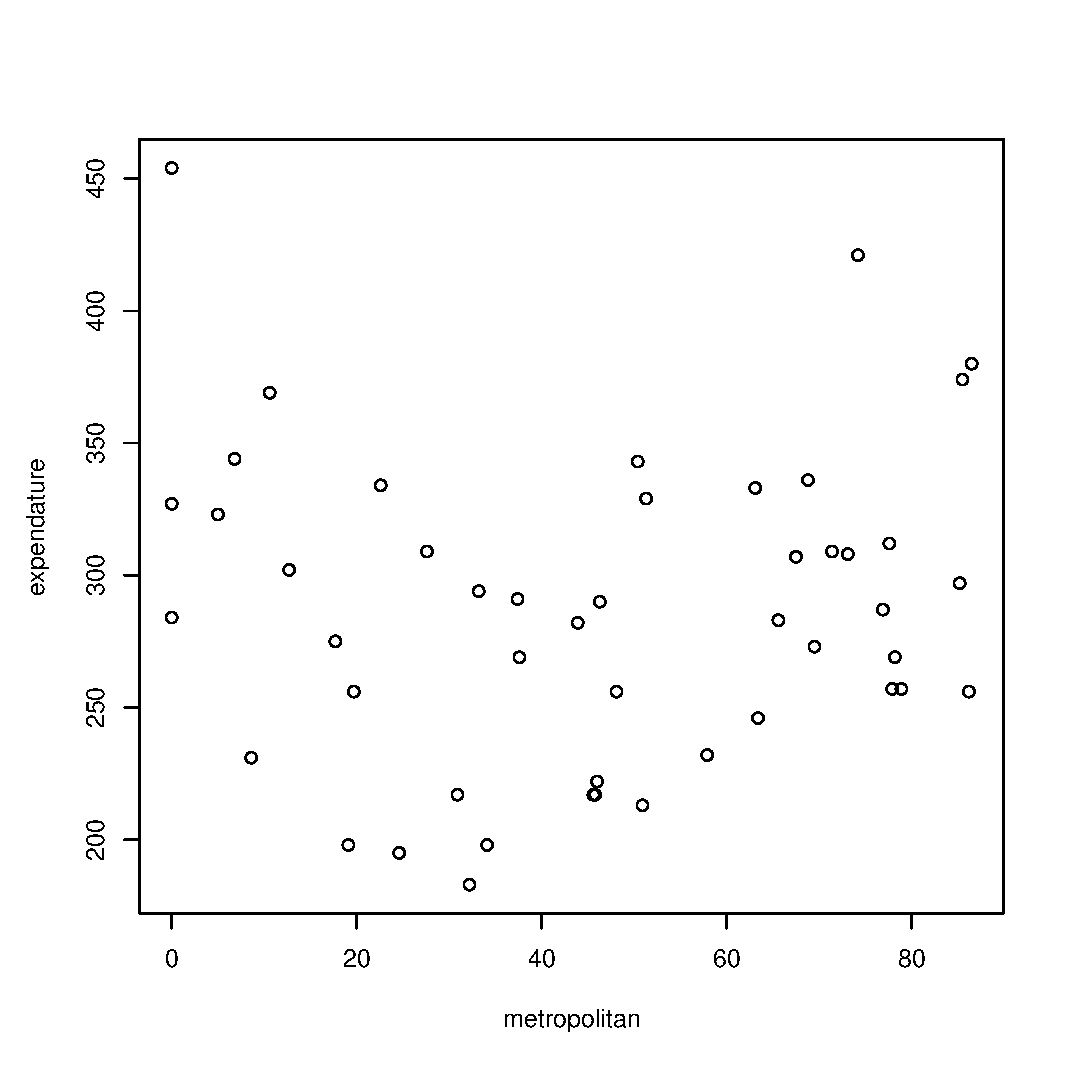
\includegraphics[width=0.5\textwidth]{share/A1_data.eps}
        \end{figure}

        The figure indicates that a linear model isn't suitable for predicting the target in this data set, no easily visible pattern can be observed in this plot. Since we are tasked with using \emph{regression trees} in this assignment, the first step is fit such a model with it, then finding the optimal number of leaves.

    \subsection*{Regression Tree Analysis}

        We have examined how a \emph{regression tree model} fits the data set using \emph{cross-validation} for finding the optimal number of \emph{leaves}. The plotted \emph{decision tree} from the fitted model can be seen in Figure~\ref{fig:tree}. This model was fitted with the following piece of \emph{R} code:

        \lstinputlisting[firstline=10,lastline=14]{../share/assignment1.r}

        \begin{figure}[h!]
            \centering
            \caption{Plotted Decision Tree for Model}
            \label{fig:tree}
            \includegraphics[width=0.5\textwidth]{example-image}
        \end{figure}

        According to the cross-validation, the optimal number of leaves is 3, which we use to prune the full tree model and get the best optimal model. These predicted results of the best model are in Figure~\ref{fig:predicted}.

        \begin{figure}[h!]
            \centering
            \caption{Plot of Metropolitan Rate \& Predict Ex}
            \label{fig:predicted}
            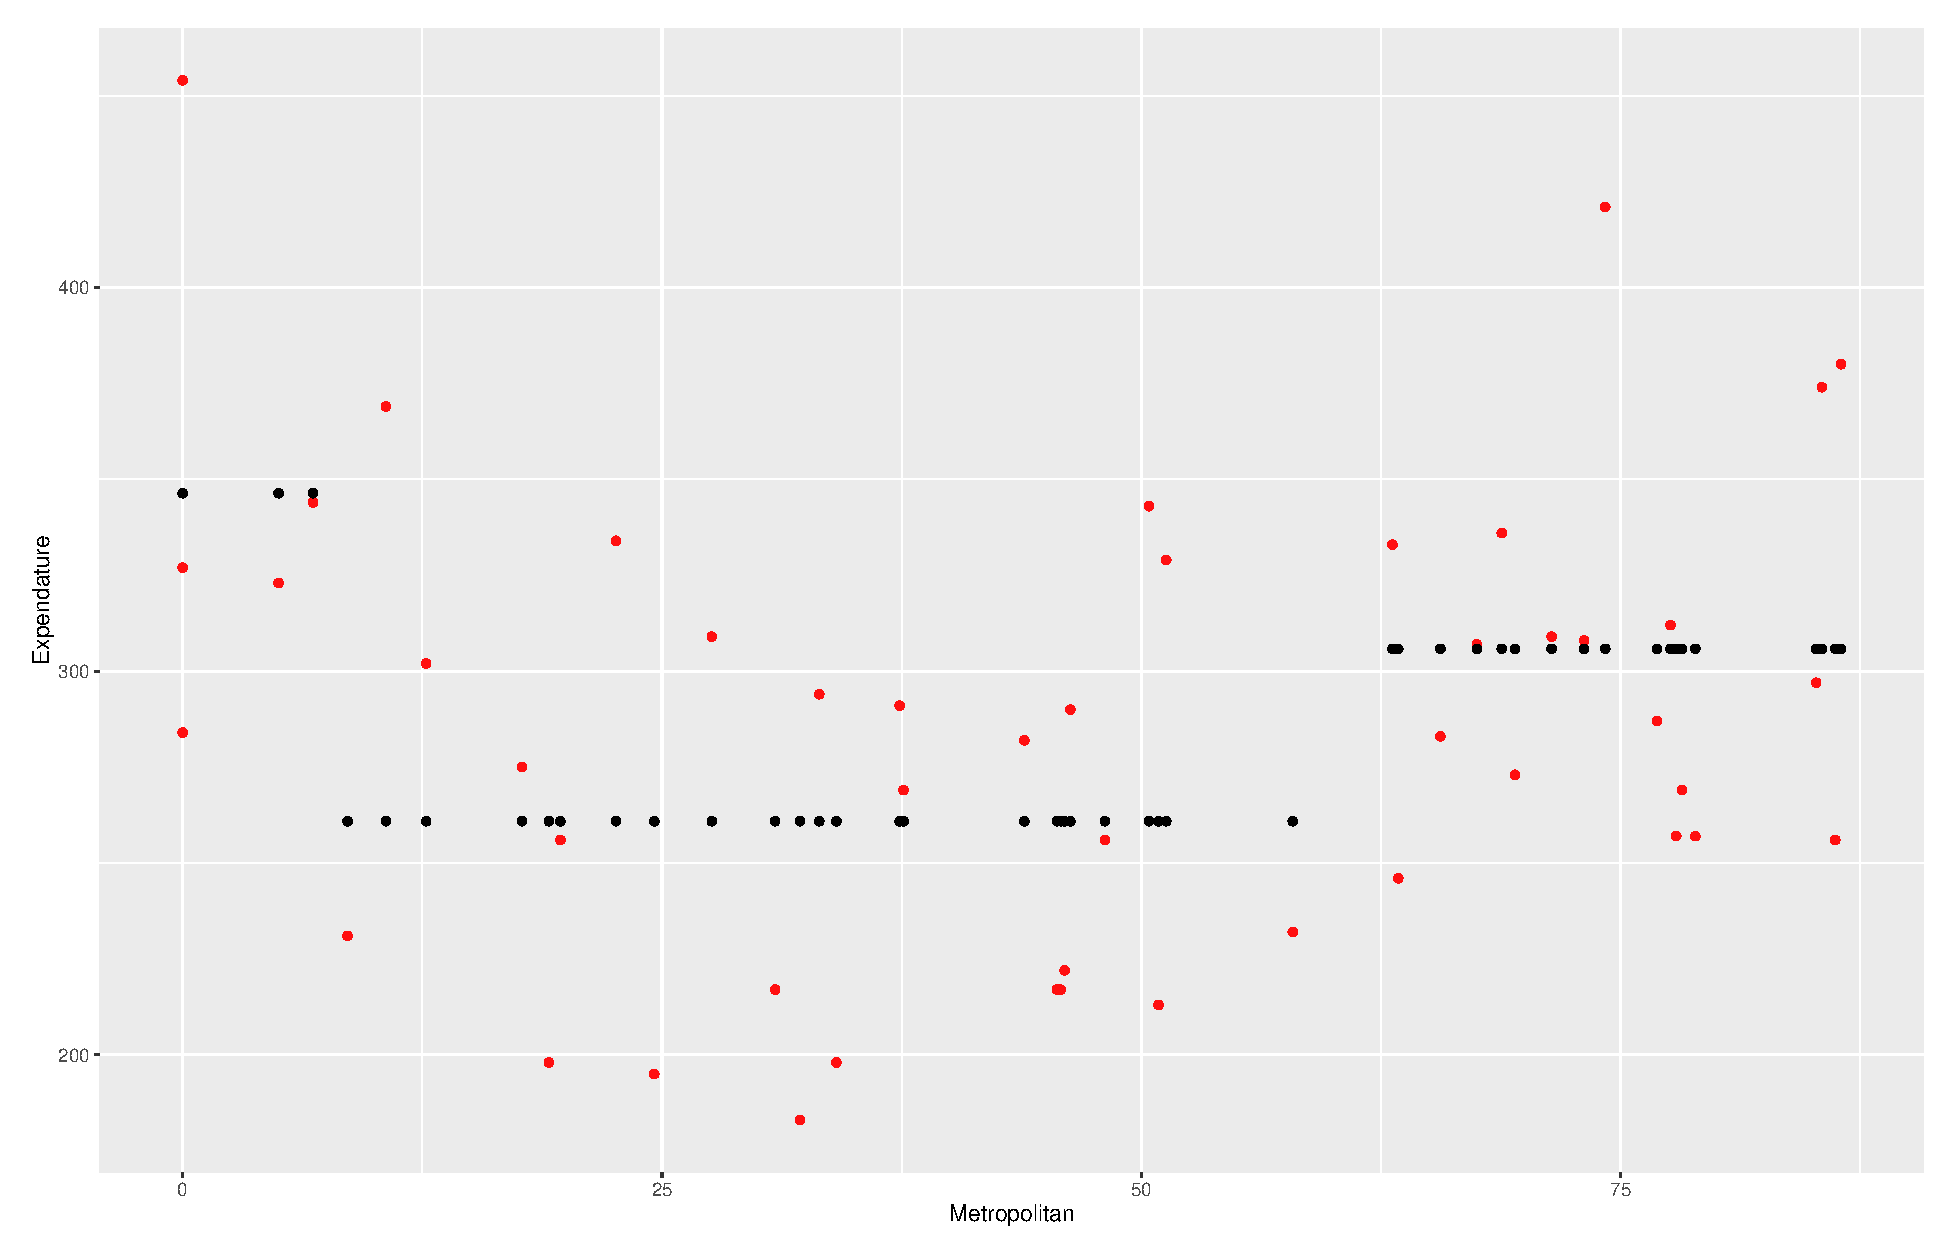
\includegraphics[width=0.5\textwidth]{share/A1_fit.eps}
        \end{figure}

        As can be seen, the predictions have less labels compared to the original data.

        The frequency of the models residuals are displayed in the histogram \ref{fig:residuals}.

        \begin{figure}[h!]
            \centering
            \caption{Histogram of the Residuals}
            \label{fig:residuals}
            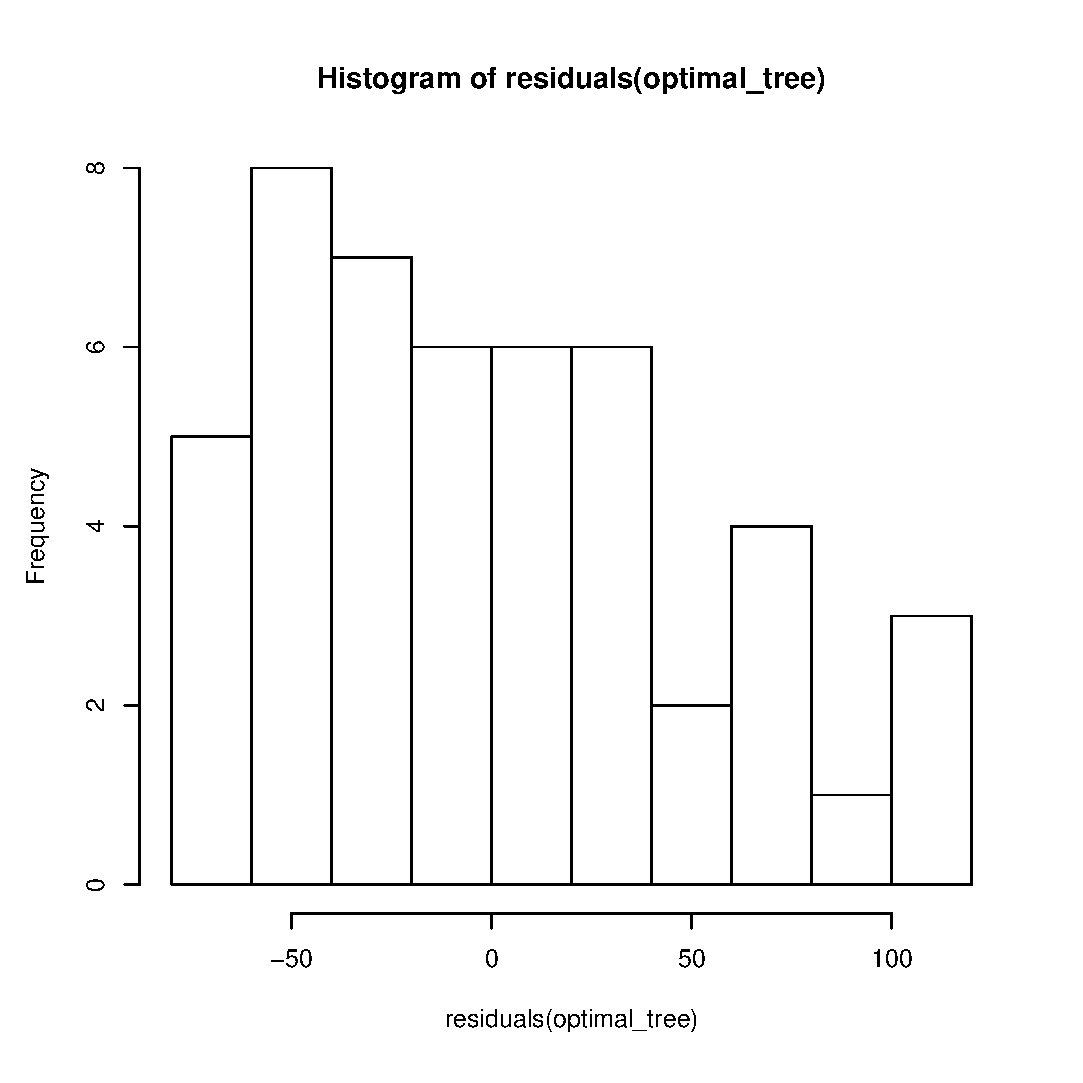
\includegraphics[width=0.5\textwidth]{share/A1_historgram_residuals.eps}
        \end{figure}

    \subsection*{Non-Parametric Bootstrap}

        We examine the same data set with a \emph{regression tree model} with \emph{non-parametric bootstrap}. The model will follow the same structure as above but use \emph{bootstrapping} instead of \emph{cross-validation}.

        The \emph{non-parametric bootstrap} re-samples the given data set $1000$ times and estimate the model based on the \emph{regression tree model}. We examine the confidence band of the predicted model with a confidence level of 0.95 (fig \ref{fig:confidence_bands}).

        \begin{figure}[h!]
            \centering
            \caption{Confidence Bands of the Regression Tree Model}
            \label{fig:confidence_bands}
            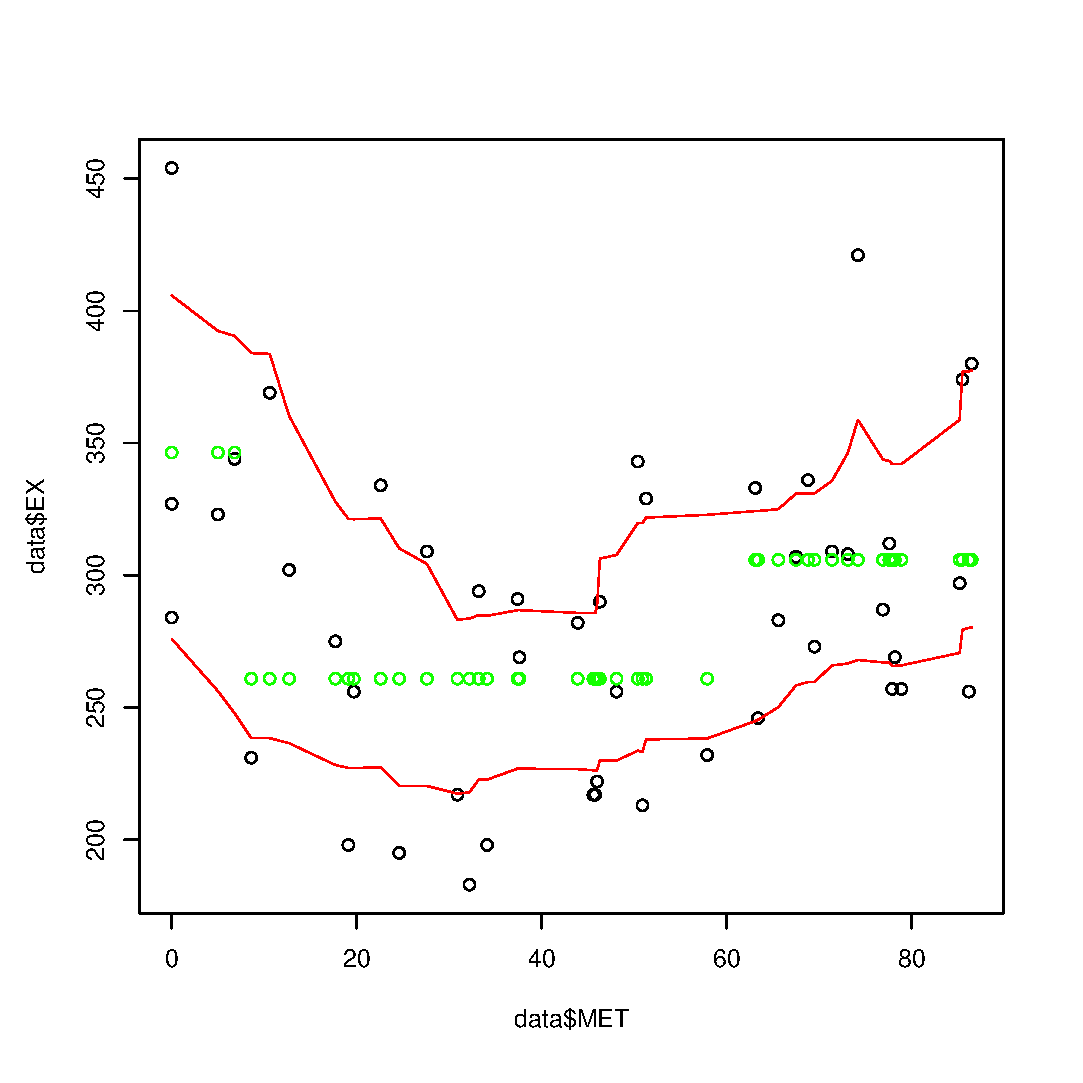
\includegraphics[width=0.5\textwidth]{share/A1_nonparametric.eps}
        \end{figure}

    \subsection*{Parametric Bootstrap}

        The preconditions as opposed to parametric bootstrap is that we know the underlying given distribution. Assuming the expenditure label as a mean given a metropolitan rate it is possible to generate additional samples to be used in the bootstrapping process. This would also require a standard deviation, which in turn can be derived from the residual data. Plotting the confidence and prediction bands give Figure~\ref{fig:confpred_bands}. In contrast to the confidence bands, prediction bands concerns the entire distribution of the data.

        \begin{figure}[h!]
            \centering
            \caption{Confidence/Prediction Bands Regression Tree Model}
            \label{fig:confpred_bands}
            \includegraphics[width=0.5\textwidth]{example-image}
        \end{figure}

        As can be seen in the figure, there are a pair of observations outside the prediction band. This is of course the result of using $95\%$ confidence.

    \section*{Assignment 2}

        In this assignment we are tasked with analyzing a data set containing observations regarding the \emph{viscosity levels} in relation with several \emph{near-infrared spectra} using \emph{PCA} and \emph{ICA} (\emph{Component Analysis Functions}).

    \subsection*{Principle Component Analysis}

        \emph{Principal Component Analysis (PCA)} is used to reduce the number of dimensions in a data set by analyzing the variance that each feature contributes to the distribution. We conduct a PCA on the given data set, this gives us the histogram in Figure~\ref{fig:pcahist}.

        \begin{figure}[h!]
            \centering
            \caption{Confidence/Prediction Bands Regression Tree Model}
            \label{fig:pcahist}
            \includegraphics[width=0.5\textwidth]{example-image}
        \end{figure}

        We observe that only two components are required to reach 99 \% cumulative variance, which are \emph{X750 (PC1)} and \emph{X752 (PC2)}. Afterwards, we plot the scores of the chosen principal components in Figure~\ref{fig:pcascore.eps}.

        \begin{figure}[h!]
            \centering
            \caption{Confidence/Prediction Bands Regression Tree Model}
            \label{fig:pcascore.eps}
            \includegraphics[width=0.5\textwidth]{example-image}
        \end{figure}

        As can be seen, there is a large amount of independence between these two components. Now we plot the loadings, which indicates the correlation between components through proportional variance. This is done in Figures~\ref{fig:x750tp}, \ref{fig:x752tp}. The outliers indicates unusual diesel fuels.

        \begin{figure}[h!]
            \centering
            \caption{Confidence/Prediction Bands Regression Tree Model}
            \label{fig:x750tp.eps}
            \includegraphics[width=0.5\textwidth]{example-image}
        \end{figure}

        \begin{figure}[h!]
            \centering
            \caption{Confidence/Prediction Bands Regression Tree Model}
            \label{fig:x752tp.eps}
            \includegraphics[width=0.5\textwidth]{example-image}
        \end{figure}

        Note the high correlation values in the same index on both plots.

        \begin{itemize}
            \item Show the data 
            \item Show the PCA function (which components were chosen?)
            \item Show the trace plot and loadings plot
            \item Questions
        \end{itemize}

    \subsection*{Independent Component Analysis}

        We perform the same analysis again, this time using the \emph{Independent component analysis} (ICA). In contrast to to PCA, where we assumed the features are correlated, we assume that they are independent. 

        The loadings are calculated with the function \( \hat{W} = K \dot W \). We plot the traces for each column (the chosen components), the result can observed in Figures~\ref{x750ical.eps}, \ref{x752ical.eps}.

        \begin{figure}[h!]
            \centering
            \caption{Confidence/Prediction Bands Regression Tree Model}
            \label{fig:x750ical.eps}
            \includegraphics[width=0.5\textwidth]{example-image}
        \end{figure}

        \begin{figure}[h!]
            \centering
            \caption{Confidence/Prediction Bands Regression Tree Model}
            \label{fig:x752ical.eps}
            \includegraphics[width=0.5\textwidth]{example-image}
        \end{figure}

        The results are quite similar to those found in PCA, but inverted.

        We now plot the scores found by doing ICA, which can be seen in Figure~\ref{fig:icascores}.

        \begin{figure}[h!]
            \centering
            \caption{Confidence/Prediction Bands Regression Tree Model}
            \label{fig:icascores.eps}
            \includegraphics[width=0.5\textwidth]{example-image}
        \end{figure}

        \begin{itemize}
            \item Show the ICA function (which components were chosen?)
            \item Show the trace and loadings plot
            \item Questions
        \end{itemize}

    \subsection*{PCA Cross-Validation}

        \begin{itemize}
            \item Show the cross validation function
            \item Show the result?
            \item Questions
        \end{itemize}

    \section*{Contributions}

    \nocite{*} % No warnings.
    \bibliographystyle{alpha}
    \bibliography{report}
    \onecolumn \appendix
    \section*{Appendix}

    \lstinputlisting[caption={Script for Assignment 1 on Bootstrapping},label={lst:assignment1}]{../share/assignment1.r}
    \lstinputlisting[caption={Script for Assignment 2 on Component Analysis},label={lst:assignment2}]{../share/assignment2.r}

\end{document}
